%=========================================================================
% (c) 2014, 2015 Josef Lusticky

\section{Benchmarking methodology}\label{sec:analysis-metodology}
Procedures described by RFC~2544 can be used to measure routing performance of the Linux kernel.
RFC~2544 specifies the benchmarking methodology for network interconnect devices.
The ideal way to implement the series of tests described in RFC~2544 is to use a tester
with both transmitting and receiving ports.
Connections are made from the sending ports of the tester to the receiving ports of the
device under test (DUT) and from the sending ports of the DUT back to the tester~\cite{rfc2544}.
Figure~\ref{fig:analysis-rfc2544} shows the test implementation.

Since the tester both sends the test traffic and receives
it back, after the traffic has been forwarded by the DUT, the tester
can easily determine if all of the transmitted packets were received~\cite{rfc2544}.
The Spirent TestCenter Application provides statistics about transmitted and received frames,
which can be used for this purpose.
\begin{figure}
	\centering
	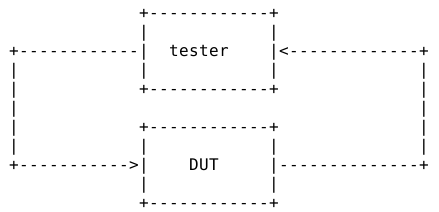
\includegraphics[width=9cm,keepaspectratio]{fig/rfc2544.png}
	\caption{RFC2544 test implementation (source:~\cite{rfc2544})}
	\label{fig:analysis-rfc2544}
\end{figure}

%=========================================================================
% (c) 2014, 2015 Josef Lusticky

\subsection{Traffic generation}\label{sub:analysis-metodology-generation}
The RFC~2544 specifies the following frame sizes to be used on Ethernet:
64, 128, 256, 512, 1024, 1280 and 1518~\cite{rfc2544}.
However, at least 66~B frame size must be used in case of transmitting UDP over IPv6 - the size of L2 header is 14,
the size of CRC is 4, the size of IPv6 header is 40 and the size of UDP header is 8.

In addition to the specified frame sizes, a custom frame size distribution can be defined for the purpose of
a real internet traffic simulation.
The Amsterdam Internet Exchange (AMS-IX) provides
statistics of the frame size distribution in the Internet traffic~\cite{amsix-frame-size}.
Figure~\ref{fig:analysis-amsix-frame-size} shows yearly frame size distribution provided by AMS-IX.
This distribution can be configured in the Spirent TestCenter Application, however,
to use the same iMix for both IPv4 and IPv6, the minimum frame size must be increased to 66 as described above.
To avoid an unfair packet scheduling by the server, all packets should be assigned the same Type of Service flag.

Unfortunately,
the provided Spirent TestCenter Application does not contain license to configure a device participating in TCP streaming.
This constraint could be workarounded by sending TCP packets with no flags set,
however such configuration is also not possible.
The generated TCP packets always contain TCP SYN flag,
which bypasses the Generic Receive Offload described in subsection~\ref{sub:linux-ingress-offloads}.
Therefore, the TCP packet processing is the same as in case of UDP.

The Spirent TestCenter Application allows to configure exact frame rate or bandwidth use.
The measurements should distinguish at least between 50~000 frames per second or 1\% of bandwidth use.
Each measurement takes 60~seconds and it is repeated 3 times.
If the kernel is able to forward all frames in at least one of the 3 measurements,
the measurement is successful.
This is to determine whether the kernel is able to forward such amount of traffic.
Some network unrelated tasks performed by the kernel may cause the inability to forward all frames,
such as gathering statistics, memory management, etc.

\begin{figure}
	\centering
	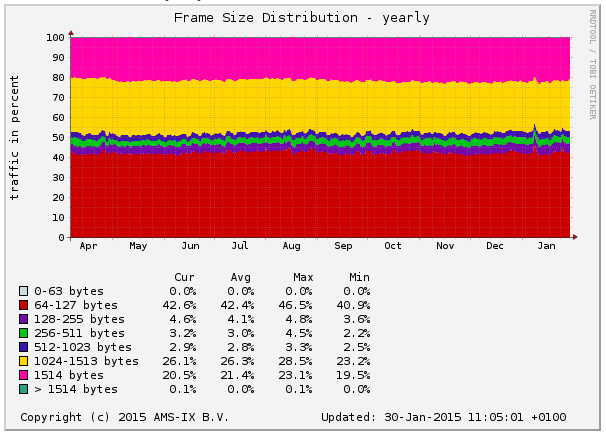
\includegraphics[width=14.5cm,keepaspectratio]{fig/amsix.png}
	\caption{Yearly frame size distribution at AMS-IX (source:~\cite{amsix-frame-size})}
	\label{fig:analysis-amsix-frame-size}
\end{figure}


%=========================================================================
% (c) 2014, 2015 Josef Lusticky

\subsection{Statistics collection}
The Spirent TestCenter Application is able to display counters of transmitted and received frames on each interface.
The counters can be used to determine whether all of the transmitted packets on one interface were received
on the other interface and hence successfully forwarded by the server.
Unfortunately, the provided Spirent TestCenter Application contains no licence to perform the RFC 2544 throughput test
automatically, so the measurements must be configured manually in the Spirent TestCenter application.
The manual configuration consists of configuring the transmit rate, observing the packet counters and comparing their values.
If the server forwards packets without a single loss, the transmit rate can be increased and the test repeated.
%Otherwise, the transmit rate must be decreased.

The proc filesystem provides access to several statistics as well.
The network statistics exported via proc filesystem can be found in the /proc/net directory.
The files in this directory are read-only and cannot be manipulated using the sysctl utility.
There are 2 important files for the measurements - the {\it{fib\_trie}} and {\it{fib\_triestat}}.
The {\it{fib\_trie}} file exports the kernel's Forwarding Information Base overview.
The file describes both the Main and Local FIBs, as described in section~\ref{sec:linux-routing}.
The {\it{fib\_triestat}} file exports metadata of the FIB trie structures,
such as average depth, maximum depth, number of leaves, etc~\cite{kernel-source}.

The CPU utilisation can be observed using the perf utility,
which can be found in the tools/perf directory of the Linux kernel source code.
Although perf is included in the Linux kernel source code,
it must be installed separately on most GNU/Linux distributions, including CentOS~7.
To obtain additional statistics, such as PCI-Express utilisation or memory utilisation,
the Intel Performance Counter Monitor (PCM)\footnote{\url{https://software.intel.com/en-us/articles/intel-performance-counter-monitor-a-better-way-to-measure-cpu-utilization}}
can be used.
The PCM package is not included in the official CentOS~7 repository,
but it can be compiled directly from the source code.
Non-maskable interrupt watchdog must be disabled
in order to run Intel PCM.
The non-maskable interrupt watchdog can be disabled by writing "0" to the /proc/sys/kernel/nmi\_watchdog file.

